\documentclass[pdftex]{beamer} 
\usepackage{graphicx}
\usepackage{amsmath,amssymb,amsthm} 
\usepackage{pb-diagram}
\usepackage{ucs}
\usepackage[utf8x]{inputenc}
%\usepackage[russian]{babel}
\usepackage{epstopdf}
\usepackage{multicol}
\usepackage{cancel}

\usepackage{amsfonts}

%%%%%%%%%%%%%%%%%%%%%%%%%%%%%%%%%%%%%%%%%%%%%%%%%%%%%%%%%%%%%%%%%%%%%%%%%%%%%%%%%%%%%%%%%%%%%%%%%%%

%\newtheorem{theorem}{Theorem}
%% \newtheorem{acknowledgement}[theorem]{Acknowledgement}
%% \newtheorem{algorithm}[theorem]{Algorithm}
%% \newtheorem{axiom}[theorem]{Axiom}
%% \newtheorem{case}[theorem]{Case}
%% \newtheorem{claim}[theorem]{Claim}
%% \newtheorem{conclusion}[theorem]{Conclusion}
%% \newtheorem{condition}[theorem]{Condition}
%% \newtheorem{conjecture}[theorem]{Conjecture}
%% \newtheorem{mycorollary}[theorem]{Corollary}
%% \newtheorem{mycriterion}[theorem]{Criterion}
%% \newtheorem{mydefinition}[theorem]{Definition}
%% \newtheorem{myexample}[theorem]{Example}
%% \newtheorem{myexercise}[theorem]{Exercise}
\newtheorem{mylemma}[theorem]{Lemma}
%% \newtheorem{mynotation}[theorem]{Notation}
%% \newtheorem{myproblem}[theorem]{Problem}
%% \newtheorem{myproposition}[theorem]{Proposition}
%% \newtheorem{myremark}[theorem]{Remark}
%% \newtheorem{mysolution}[theorem]{Solution}
%% \newtheorem{mysummary}[theorem]{Summary}
%% \newenvironment{myproof}[1][Proof]{\textbf{#1.} }{\ \rule{0.5em}{0.5em}}


\newcommand{\go}{\stackrel{\circ }{\mathfrak{g}}}
\newcommand{\ao}{\stackrel{\circ }{\mathfrak{a}}}
\newcommand{\co}[1]{\stackrel{\circ }{#1}}
\newcommand{\pia}{\pi_{\mathfrak{a}}}
\newcommand{\piab}{\pi_{\mathfrak{a}_{\bot}}}
\newcommand{\gf}{\mathfrak{g}}
\newcommand{\gfh}{\hat{\mathfrak{g}}}
\newcommand{\af}{\mathfrak{a}}
\newcommand{\afh}{\hat{\mathfrak{a}}}
\newcommand{\bff}{\mathfrak{b}}
\newcommand{\afb}{\mathfrak{a}_{\bot}}
\newcommand{\hf}{\mathfrak{h}}
\newcommand{\hfg}{\hf_{\gf}}
\newcommand{\hfb}{\mathfrak{h}_{\bot}}
\newcommand{\pf}{\mathfrak{p}}
\newcommand{\aft}{\widetilde{\mathfrak{a}}}
\newcommand{\sfr}{\mathfrak{s}}
%\pagestyle{plain}

\theoremstyle{definition} \newtheorem{Def}{Definition}
\setbeamertemplate{caption}[empty]
\newcommand{\tr}{\hat\triangleright} \newcommand{\trc}{\triangleright}
\newcommand{\adk}{a^{\dagger}_{\kappa}} \newcommand{\ak}{a_{\kappa}}
\def\bF{\mbox{$\overline{\cal F}$}} \def\F{\mbox{$\cal F$}}

%\usetheme{AnnArbor}
\usetheme[everytitleformat=regular]{m}


\title[Dimer model]{Free energy scaling in dimer model}

\author[A. Nazarov]{A. Nazarov}

\institute[SPbSU]{
  Department of High Energy and Elementary Particle Physics\\
  faculty of physics\\
  St Petersburg State University\\
  198904, St Petersburg, Russia\\
  e-mail: a.a.nazarov@spbu.ru
}

\date[MQFT 2018] % (optional, should be abbreviation of conference name)
{27.08.2018}
\begin{document}
\maketitle

\section{Introduction}

\begin{frame}
  \frametitle{Abstract}

  We consider dimer model on a hexagonal lattice. This model can be seen as a ``pile of cubes in the
  corner''. The partition function is given by the determinant of Kasteleyn matrix. We use the
  expression for the partition function to derive the scaling behavior of free energy in the limit
  of lattice mesh tending to zero and temperature tending to infinity. We discuss the connection of
  the expansion coefficients to the geometry of the domain.

\end{frame}
\section{Dimer model}
\begin{frame}
  \frametitle{Model definition}
  Dimers -- pairings on bipartite graph.
  
  We consider hexagonal lattice. 
  \begin{figure}
    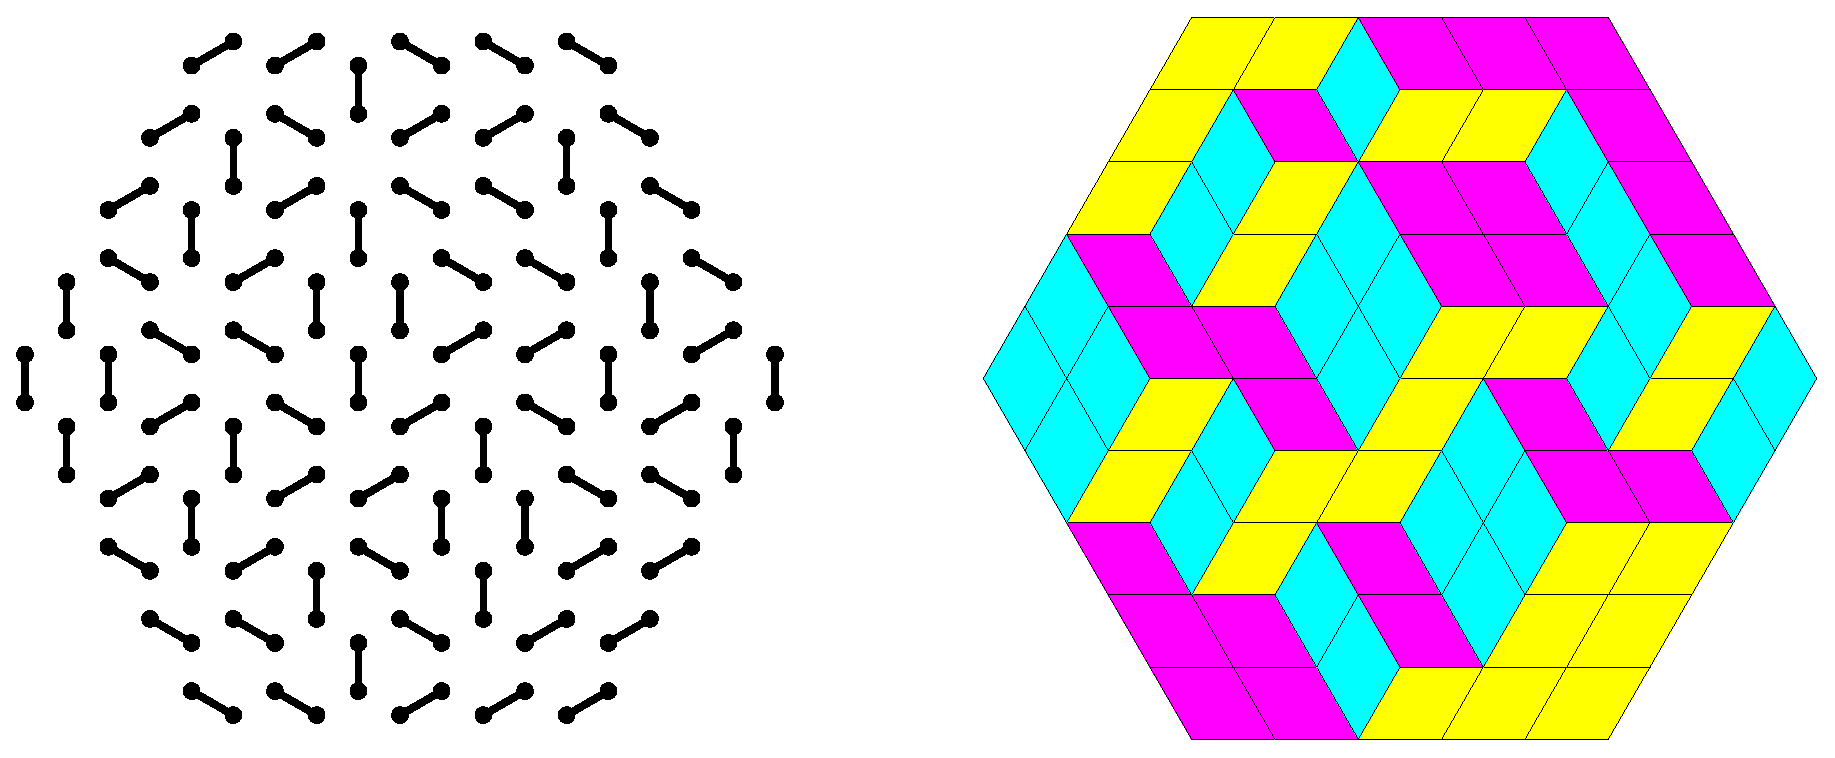
\includegraphics[scale=0.35]{loz}
    \caption{\label{dhf}A configuration of dimers on the hexagonal lattice and a corresponding picture of ``cubes in the corner''.}
  \end{figure}
\end{frame}
\begin{frame}
  \frametitle{Energy and partition function}
  Energy of configuration is given by the volume of cubes:
    \begin{equation}
    \label{eq:10}
    E[\mathrm{conf}]=\mathrm{Volume}
  \end{equation}
  The partition function:
  \begin{equation}
    \label{eq:14}
    Z[q]=\sum_{\mathrm{conf}} e^{-\frac{E[\mathrm{conf}]}{T}}=\sum_{\mathrm{conf}}q^{-\mathrm{Vol}[\mathrm{conf}]}=\sum_{\mathrm{conf}}e^{-\frac{\mathrm{Vol[conf]}}{T}}
  \end{equation}
  On on a hexagonal domain with sides $M,N,K$ it is given by MacMahon formula :
  \begin{equation}
    \label{eq:12}
       Z[M,N,K,q]=\prod_{i=1}^{M}\prod_{j=1}^{N}\prod_{k=1}^{K}\frac{1-q^{i+j+k-1}}{1-q^{i+j+k-2}}
  \end{equation}

\end{frame}
\begin{frame}
  \frametitle{Kasteleyn matrix and Dirac operator}
%%  Consider infinite-dimensional graded algebra, e.g. $\gf[[t]]$ or $\hat\gf$

  $K(w,b)$ -- weighted adjacency matrix, $K(w,b)\sim w-b\in \mathbb{C}$

  MacMahon formula is obtained if for adjacent $b\sim w$:
  \begin{eqnarray}
    \label{eq:18}
    K(w,b)=q^{\Re w+\Im w} \quad \mathrm{if}\quad \Im w=\Im b\\
    K(w,b)=1 \quad \mathrm{if}\quad \Im w\neq\Im b
  \end{eqnarray}

  \begin{equation}
    \label{eq:15}
    Z=\sum_{\mathrm{conf}}\prod_{e\in \mathrm{conf}}w(e)=|\det K|
  \end{equation}
  Discrete Dirac operator in vertex $v$:
  \begin{equation}
    \label{eq:16}
    (Kf)(v)=\sum_{u}K(v,u) f(u)
  \end{equation}
  Mean curvature $\sim$ mean energy per site

  Continuous (scaling) limit?
\end{frame}
\begin{frame}
  \frametitle{Free energy scaling}
  Free energy
  \begin{equation}
    \label{eq:17}
    \frac{f}{T}=-\frac{1}{V}\ln Z(M,N,K,q)
  \end{equation}
  where $V$ -- \# of dimers = \# of cube faces = $\frac{1}{2}\cdot$ \# of vertices
  \begin{equation}
    \label{eq:19}
    V=MN+NK+MK
  \end{equation}
  Scaling limit:
  \begin{eqnarray}
    \label{eq:20}
    T\to \infty, \quad M,N,K\to \infty\\
    \frac{M}{T}=a,\quad \frac{N}{T}=b, \quad \frac{K}{T}=c\\
        \varepsilon=\frac{1}{T}\to 0
  \end{eqnarray}

\end{frame}
\section{Free energy scaling}
\label{sec:free-energy-scaling}


\begin{frame}
  \frametitle{Expanding free energy}
  \begin{equation}
    \label{eq:1}
     -\frac{f}{T}=\frac{1}{V}\ln Z = \sum_{i=1}^{M} \sum_{j=1}^{N} \sum_{k=1}^{K} \frac{1}{V}
  \ln\left(\frac{1-e^{-\varepsilon (i+j+k)} e^{\varepsilon}}{1-e^{-\varepsilon (i+j+k)} e^{2\varepsilon}}\right)
\end{equation}
Expanding exponents $e^{\varepsilon}, e^{2\varepsilon}$ in power series and combining the logarithms we get:
\begin{multline}
  \label{eq:2}
   -\frac{f}{T}= \sum_{i=1}^{M} \sum_{j=1}^{N} \sum_{k=1}^{K} \frac{1}{V}\left\{
    \ln\left(1-\frac{1}{e^{\varepsilon(i+j+k)}-1}\sum_{l=1}^{\infty} \frac{\varepsilon^{l}}{l!}\right)-\right.\\
  -\left.\ln\left(1-\frac{1}{e^{\varepsilon(i+j+k)}-1}\sum_{l=1}^{\infty} \frac{2^{l}\varepsilon^{l}}{l!}\right)\right\}
\end{multline}
Denote
\begin{equation}
  \label{eq:5}
  g(x,y,z)=\frac{1}{e^{x+y+z}-1}
\end{equation}
\end{frame}
\begin{frame}
  \frametitle{Expansion to third term}
Then expand the logarithms up to $\varepsilon^{3}$:
\begin{multline}
  \label{eq:4}
  \frac{f}{T}=- \sum_{i=1}^{M} \sum_{j=1}^{N} \sum_{k=1}^{K} \frac{1}{V}\left\{
    g(i\varepsilon,j\varepsilon,k\varepsilon)+\frac{3}{2}\varepsilon\left[g(i\varepsilon,j\varepsilon,k\varepsilon)+g(i\varepsilon,j\varepsilon,k\varepsilon)^{2}\right]\right.\\
  \left.+\frac{7}{6}\varepsilon^{2}\left[g(i\varepsilon,j\varepsilon,k\varepsilon)+3 g(i\varepsilon,j\varepsilon,k\varepsilon)^{2}+2 g(i\varepsilon,j\varepsilon,k\varepsilon)^{3}\right]\right\}  
\end{multline}
Looks like Riemann sums, but we need corrections in $\varepsilon$ as $\varepsilon\to 0$.

Use the approximation formula for integral of some function $\tilde{f}$:
\begin{multline}
  \label{eq:21}
  \int_{0}^{a} \int_{0}^{b}\int_{0}^{c}\tilde{f}(x,y,z) dx\; dy\;
  dz\approx\sum_{i=1}^{M}\sum_{j=1}^{N}\sum_{k=1}^{K}\left\{\varepsilon^{3}\tilde{f}\left(i\varepsilon,j\varepsilon,k\varepsilon\right)-\right.\\
  \left.-\left[\frac{\varepsilon^{4}}{2}\left((\partial_{x}+\partial_{y}+\partial_{z})\tilde{f}\right)(i\varepsilon,j\varepsilon,k\varepsilon)\right]+\right.\\
  \left.\varepsilon^{5}\left(\frac{1}{6}(\partial_{x}^{2}+\partial_{y}^{2}+\partial_{z}^{2})+\frac{1}{4}(\partial_{x}\partial_{y}+\partial_{x}\partial_{z}+\partial_{y}\partial_{z})\right)\tilde{f}\left(i\varepsilon,j\varepsilon,k\varepsilon\right)  \right\}
\end{multline}
\end{frame}

\begin{frame}
  \frametitle{Integral representation and singularity}
  Note that $\partial_{x}g(x,y,z)=-g(x,y,z)-g(x,y,z)^{2}$.
  Use integral representation for the $1^{st}$ term, get corrections to the higher terms:
  \begin{multline*}
    \frac{f}{T}=-\frac{1}{ab+bc+ca}\left\{\int_{0}^{a} \int_{0}^{b}\int_{0}^{c}\frac{dx dy dz}{e^{x+y+z}-1}+\right.\\
    \left.+\sum_{i=1}^{M}\sum_{j=1}^{M}\sum_{k=1}^{M}\frac{\varepsilon^{5}}{12}\left[g(i\varepsilon,j\varepsilon,k\varepsilon)+3 g(i\varepsilon,j\varepsilon,k\varepsilon)^{2}+2 g(i\varepsilon,j\varepsilon,k\varepsilon)^{3}\right]\right\}
  \end{multline*}
  No singularity in the sum, but $\int_{0}^{a} \int_{0}^{b}\int_{0}^{c}\frac{dx dy dz}{(\exp(x+y+z)-1)^{3}}$ diverges logarithmically.
  We can subtract and add $\frac{1}{i\varepsilon}$. Also:
  \begin{equation}
    \label{eq:24}
    \sum_{i=1}^{M}\frac{1}{i}=\frac{1}{M}\sum_{i=1}^{M}\frac{1}{i/M}=\int_{\frac{1}{M}}^{1}\frac{dx}{x}+\gamma+O(\varepsilon)=-\ln\varepsilon+\ln a+\gamma+O(\varepsilon)
  \end{equation}

\end{frame}
\begin{frame}
  \frametitle{Final result}
  \begin{multline*}
    \frac{f}{T}=-\frac{1}{ab+bc+ca}\left\{\int_{0}^{a} \int_{0}^{b}\int_{0}^{c}\frac{dx dy dz}{e^{x+y+z}-1}+\right.\\
    \left.+\frac{\varepsilon^{2}}{12}\int_{0}^{a} \int_{0}^{b}\int_{0}^{c}\left(\frac{e^{2(x+y+z)}+e^{x+y+z}}{\left(e^{x+y+z}-1\right)^{3}}-\frac{1}{bc}\frac{1}{x}\right)dx dy dz+\right.\\
    \left.+\frac{\varepsilon^{2}}{12}(\ln a-\gamma)+\frac{\varepsilon^{2}}{12}\ln \varepsilon\right\}    
  \end{multline*}
  Second integral can be taken explicitly:
  \begin{multline*}
    \frac{f}{T}=-\frac{1}{ab+bc+ca}\left\{\int_{0}^{a} \int_{0}^{b}\int_{0}^{c}\frac{dx dy dz}{e^{x+y+z}-1}+\right.\\
    \left.+\frac{\varepsilon^{2}}{12}\left[\ln\left(\frac{(e^{a}-1)(e^{b}-1)(e^{c}-1)(e^{a+b+c}-1)}{(e^{a+b}-1)(e^{b+c}-1)(e^{a+c}-1)}\right)-\gamma\right]+\frac{\varepsilon^{2}}{12}\ln \varepsilon\right\}    
  \end{multline*}
\end{frame}
\begin{frame}
  \frametitle{Conclusion}
  \begin{itemize}
  \item This free energy scaling formula is in agreement with numerical computations
  \item There are Monte-Carlo simulation results that support this scaling
  \item Form of our formula is similar to the asymptotics of discrete Dirac operator obtained by Kenyon
  \end{itemize}
\end{frame}

\begin{frame}
  \frametitle{Thank you!}
\end{frame}

\end{document}
